% !TEX root = ./Vorlesungsmitschrift DIFF 2.tex  
\lecture{Mo 25.05. 10:15}{}
\section*{Taylor-Formel, lokale Extrema}
\begin{notation}[Multi-Index-Schreibweise]
  Sei \( \alpha\definedas(\alpha_1,\dotsc,\alpha_n)\in \naturals_{0}^n \). Dann definiert man
  \begin{align*}
    \abs{\alpha}&\definedas\alpha_1+\alpha_2+\dotsb+\alpha_n\\
    \factorial{\alpha}&\definedas \factorial{\alpha_1}\factorial{\alpha_2}\dotsb\factorial{\alpha_n}.
  \end{align*}
  Ist \( x=\transpose-{(x_1,\dotsc,x_n)}\in \reals^n \), so setzt man 
  \begin{equation*}
    x^{a}\definedas x_1^{\alpha_1}x_2^{\alpha_2}\dotsb x_n^{\alpha_n}.
  \end{equation*}
  Ist \( f \) eine \( \abs{\alpha} \)-mal stetig differenzierbare Funktion, so ist 
  \begin{equation*}
    \partial^{\alpha}f\definedas \partial_1^{\alpha_1}\partial_2^{\alpha_2}\dotsb\partial_n^{\alpha_n}f
  \end{equation*}
\end{notation}
\begin{lemma}\label{funktion_entlang_gerade_ableitung}
  Sei \( f\maps U\to \reals \), \( U\subset \reals^n \) offen, ine \( k \)-fach stetig differenzierbare Funktion. Sei \( a\in U \) und sei \( h\in \reals^n \) so, dass \( \set{a+th|tt\in \interval{0}{1}} \) ganz in \( U \) liegt.
  \begin{figure}[H]
    \centering
    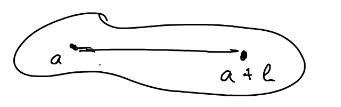
\includegraphics[width=0.5\linewidth]{verbindungsstrecke_in_umgebung}
    \label{fig:verbindungsstrecke_in_umgebung}
  \end{figure}
  Dann ist die Funktion \( g\maps \interval{0}{1}\to \reals \), \( g(t)=f(a+th) \) \( k \)-mal stetig differenzierbar und es gilt 
  \begin{equation*}
    g^{(k)}(t)=\sum_{\explain{\text{Summe über alle \( \alpha=(\alpha_1,\dotsc,\alpha_n)\in \naturals_0^h \) mit \( \alpha_1+\alpha_2+\dotsb+\alpha_n=k \)}}{\abs{\alpha}=k}}\frac{\factorial{k}}{\factorial{\alpha}}\partial^{\alpha}f(a+th)h^{\alpha}.
  \end{equation*}
\end{lemma}
\begin{proof}
  \begin{proofenumerate}
    \item Wir zeigen per Induktion über \( k \), dass gilt
    \begin{equation*}
      g^{(k)}(t)=\sum_{\mathclap{i_1,\dotsc,i_k\in \set{1,\dotsc,n}}}\partial_{i_1}\dotsb\partial_{i_k} f(a+th)h_{i_1}\dotsb h_{i_k}.
    \end{equation*}
    \begin{proofdescription}
      \item[Induktionsanfang: \( k=1 \)]
      \begin{align*}
        g'(t)&=Df(a+th)\matrixmult h\eqstep[p,v=false]{\text{Kettenregel}}\\
        &\sum_{i=1}^{n}\partial_i f(a+th) h_i.
      \end{align*}
      \item[\( k-1\to k \)]\Style{DDisplayFunc=outset}
      \begin{equation*}
        \D{\parens*{\sum_{i_1,\dotsc,i_{k-1}\in \set{1,\dotsc,n}}\partial_{i_1}\dotsb \partial_{i_{k-1}}f(a+th)h_{i_1}\dotsb h_{i_{k-1}}}}{t}=\sum_{i_1,\dotsc,i_{k-1}\in \set{1,\dots,n}} \sum_{i=1}^{n}\partial_i \partial_{i_1}\dotsc \partial_{i_{k-1}} f(a+th) h_{i_1}\dotsb h_{i_{k-1}}h_i.
      \end{equation*} 
    \end{proofdescription}
    \item Kommt unter den Indizes \( (i_1k,\dotsc,i_k) \) der Index \( 1 \) \( \alpha_1 \)-mal vor, der Index \( 2 \) \( \alpha_2 \)-mal,\dots, der Index \( n \) \( \alpha_n \)-mal, so ist 
    \begin{equation*}
      \partial_{i_1}\dotsb\partial_{i_k} f(a+th)=\partial_1^{\alpha_1}\dotsc \partial_n^{\alpha_n}f(a+th).
    \end{equation*}
    Es gibt 
    \begin{equation*}
      \frac{\factorial{k}}{\factorial{\alpha_1}\dotsb \factorial{\alpha_n}}
    \end{equation*}
    \( k \)-Tupel \( (i_1,\dotsc,i_k) \) von Zahlen \( 1\leq i_j\leq n \), in denen \( 1 \) genau \( \alpha_1 \)-mal, \( 2 \) genau \( \alpha_2 \)-mal, \dots, \( n \) genau \( \alpha_n \)-mal vorkommt (ohne Beweis). \timplies \Beh.
  \end{proofenumerate}
\end{proof}
\begin{satz}[Taylorsche Formel]
  Sei \( f\maps U\to \reals \), \( U\subset \reals^n \) offen, \( (k+1) \)-mal stetig differenzierbar. Sei \( a\in U \) und \( h\in \reals^n \) \sd \( \set{a+tht|t\in \interval{0}{1}}\subset U \). Dann existiert \( \theta\in \interval{0}{1} \) \sd
  \begin{equation*}
    f(a+h)=\sum_{\substack{\abs{\alpha}\leq k\\ \alpha\in \naturals_0^n}}\frac{1}{\factorial{\alpha}} \partial^{\alpha} f(a) h^{\alpha} +\sum_{\substack{\abs{\alpha}=k+1\\ \alpha\in \naturals_0^{n}}} \frac{1}{\factorial{\alpha}} \partial^{\alpha} f(a+\theta h) h^{\alpha}.
  \end{equation*}
\end{satz}
\begin{proof}
  Setze \( g\maps \interval{0}{1}\to \reals \), \( g(t)\definedas f(a+th) \). Taylorsche Formel aus der \diffcourse{1} \timplies \texists \( \theta\in \interval{0}{1} \) \sd
  \begin{equation*}
    g(1)=\sum_{j=0}^{k}\equalto{(\ref{funktion_entlang_gerade_ableitung})\logicspace \sum_{\abs{\alpha}=j}\frac{1}{\factorial{\alpha}}\partial^{\alpha}f(a)h^{\alpha}}{\underbrace{\frac{1}{\factorial{j}}g^{(j)}(0)}}+\equalto[Big]{\sum_{\abs{\alpha}=k+1}\frac{1}{\factorial{\alpha}}f(a+\theta h)h^{\alpha}}{\underbrace{\frac{1}{\factorial+{k+1}}g^{(k+1)}(\theta)}}.
  \end{equation*}
\end{proof}
\begin{folgerung}
  Sei \( f\maps U\to \reals \), \( U\subset \reals^n \) offen, \( k \)-mal stetig differenzierbar. Sei \( a\in U \) und \( \delta>0 \) \sd \( B_{\delta}(a)\subset U \). Dann gilt für alle \( h\in B_{\delta}(0) \):
  \begin{equation*}
    f(a+h)=\sum_{\alpha\leq k}\frac{1}{\factorial{\alpha}} \partial^{\alpha} f(a) h^{\alpha}+ R_{k,a}(h)
  \end{equation*}
  mit \( \frac{R_{k,a}(h)}{\norm{h}^k}\goesto 0 \) für \( h\goesto 0 \). 

  Äquivalent:
  \begin{equation*}
    f(x)=\sum_{\alpha\leq k}\frac{1}{\factorial{\alpha}} \partial^{\alpha} f(a) (x-a)^{\alpha}+ R_{k,a}(x-a)
  \end{equation*}
  für \( x\in B_{\delta}(a)\). \emph{\enquote{Taylor-Entwicklung bis zur Ordnung \( k \) mit Entwicklungspunkt \( a \)}}.
\end{folgerung}
\begin{proof}
  \texists \( \theta=\alpha_{a,h}\in \interval{0}{1} \) \sd
  \begin{align*}
    f(a+h)&=\sum_{\abs{\alpha}\leq k-1}\frac{1}{\factorial{\alpha}} f(a) h^{\alpha}+\sum_{\abs{\alpha}}\partial^{\alpha} f(a+\theta h)h^{\alpha}\\
    &=\sum_{\abs{\alpha}\leq k}\frac{1}{\factorial{\alpha}} \partial^{\alpha}f(a) h^{\alpha}+\sum_{\abs{\alpha}=k}\frac{1}{\factorial{\alpha}}\parens{\underbrace{\partial^{\alpha}f(a+\theta h)-\partial^{\alpha}f(a)}_{\definedas r_{\alpha,a}(h)}}h^{\alpha}.
  \end{align*}
  \( \partial^{\alpha} f \) ist stetig \timplies \( r_{\alpha,a}(h)\goesto r_{\alpha,a}(0)=0 \) für \( h\goesto 0 \) für \( h\goesto 0 \). Setze 
  \begin{equation*}
    R_{k,a}(h)\definedas \sum_{\abs{\alpha}=k}\frac{1}{\factorial{\alpha}} r_{\alpha,a}(h) h^{\alpha},
  \end{equation*}
  dann gilt \( \frac{R_{k,\alpha}(h)}{\norm{h}^k}\goesto 0 \), denn
  \begin{equation*}
    \frac{\abs{h^\alpha}}{\explicitnorm{\max}{h}^k}=\frac{\abs{h_1}^{\alpha_1}\dotsb \abs{h_n}^{\alpha_n}}{\parens*{\explicitnorm{\max}{h}}^k}\leq 1
  \end{equation*}
  für \( \abs{\alpha}=\alpha_1+\dotsb+\alpha_n=k \).
  
\end{proof}

\begin{notation*}
  \begin{equation*}
    P_m(h)\definedas P_{m,a}(h)=\sum_{\abs{\alpha}=m}\frac{1}{\factorial{\alpha}} \partial^{\alpha} f(a) h^{\alpha}
  \end{equation*}
  ist ein homogenes Polynom von Grad \( m \) (in \( h \)), das sogenannte \emph{Taylorpolynom} zu \( f \) zum Entwicklungspunkt \( a \). Es gilt
  \begin{equation*}
    f(a+h)=\sum_{m=0}^k P_{m,a}(h)+R_{k,a}(h).
  \end{equation*}
\end{notation*}
\begin{description}
  \item[\( m=0 \)] \( P_0(h)=f(a)\) konstant.
  \item[\( m=1 \)] Die Summe läuft über alle
  \begin{equation*}
    (\alpha_1,\dotsc,\alpha_n)\in \Set{(1,0,\dotsc,0),(0,1,0,\dotsc),\dotsc,(0,\dotsc,0,1)}.
  \end{equation*}
  Also gilt
  \begin{equation*}
    P_1(h)=\sum_{j=1}^{a} \partial_j f(a) h_j=\begin{pNiceMatrix} \partial_1 f(a) & \Cdots & \partial_n f(a) \end{pNiceMatrix}\matrixmult h.
  \end{equation*}
  Die Formel aus der Folgerung entspricht also genau der linearen Approximation von \( f \), die durch Ableitung gegeben ist.
  \item[\( m=2 \)] Die Summe läuft über alle
  \begin{multline*}
    (\alpha_1,\alpha_2,\dotsc,\alpha_n)\in\{ (1,1,0,\dotsc,0),(1,0,1,0,\dotsc,0),\dotsc\\
    ,(0,1,1,0,\dotsc,0),(0,1,0,1,0,\dotsc,0),\dotsc\\
    ,\dotsc\\
    ,(2,0,\dotsc,0),(0,2,0,\dotsc,0),\dotsc,(0,\dotsc,0,2)\}.
  \end{multline*}
  Also ist
  \begin{equation*}
    P_2(h)=\underbrace{\sum_{j=1}^{n}\sum_{i=j+1}^{n}\partial_i \partial_j f(a) h_i h_j}_{\mathclap{=\sum_{j<i}\partial_i \partial_j f(a) h_i h_j\explain{\text{\hyperlink{schwarzscher_satz}{Schwarz}}}{=}\frac{1}{2}\sum_{i\neq j}\partial_i \partial_j f(a) h_i h_j}}+\sum_{j=1}^n\frac{1}{2}\partial_j^2 f(a) h_j^2=\frac{1}{2}\sum_{i,j}\partial_j \partial_i f(a) h_i h_j.
  \end{equation*}
  Man definiert daher die sogenannte \emph{Hesse-Matrix}
  \begin{equation*}
    H_f(a)\definedas \parens*(\partial_i \partial_j f(a))_{\substack{i\in \set{1,\dotsc,n}\\j\in \set{1,\dotsc,n}}}
  \end{equation*}
  und schreibt
  \begin{equation*}
    \boxed{f(a+h)=f(a)+\scalarproduct{\grad-{f}(a)}{h}+\frac{1}{2}\scalarproduct{h}{H_f(a) h}}+R_{z,a}(h)
  \end{equation*}
  für \( f\maps U\to \reals \) zweimal stetig differenzierbar und \( h\in B_{\delta}(0) \), \( \delta>0 \) \sd \( B_{\delta}(a)\subset U \).
\end{description}
\section*{Lokale Extrema}
Wir hatten in \ref{extremum_notwendige_bedingung} bereits gesehen: Ist \( a\in U \) lokale Extremstell von \( f\maps U\to \reals \), \( U\subset \reals^n \) offen, differenzierbar, so ist \( \grad-{f}(a)=0 \).
\begin{satz}\label{hinreichende_bedingung_isoliertes_extremum}
  Sei \( f\maps U\to \reals \) zweimal stetig differenzierbar, \( U\subset \reals^n \) offen. Sei \( a\in U \) \sd \( \grad-{f}(a)=0 \). Dann gilt:
  \begin{eigenschaftenenumerate}
    \item\label{hinreichende_bedingung_isoliertes_minimum} Ist \( H_f(a) \) positiv definit (\dh \( \scalarproduct{h}{H_f(a)h}>0 \) \tforall \( h\in \reals^n \), \( h\neq 0 \)), so hat \( f \) in \( a \) ein lokales (isoliertes) Minimum.
    \item\label{hinreichende_bedingung_isoliertes_maximum} Ist \( H_f(a) \) negativ definit (\dh \( \scalarproduct{h}{H_f(a)}<0 \) \tforall \( h\neq 0 \)), so hat \( f \) in \( a \) ein lokales (isoliertes) Maximum.
    \item\label{hinreichende_bedingung_kein_extremum} Ist \( H_f(a) \) indefinit (\dh \texists  \( h \) \sd \( \scalarproduct{h}{H_f(a)h}>0 \) \emph{und} \texists \( \tilde{h} \) \sd \( \scalarproduct{\tilde{h}}{H_f(a)\tilde{h}}<0 \)), so hat \( f \) in \( a \) kein lokales Extremum.
  \end{eigenschaftenenumerate}
\end{satz}
\begin{bemerkung*}
  Ist \( H_f(a) \) positiv oder negativ \emph{semi}definit \sd \tforall \( h\neq 0 \) ist \( \scalarproduct{h}{H_f(a)h}\geq 0 \) (\bzw \( \leq 0 \)), so ist keine allgemeine Aussage möglich.
\end{bemerkung*}
\begin{beispiel*}
  \( f_1(x,y)=x^2+y^4 \), \( f_2(x,y)=x^2 \), \( f_3(x,y)=x^2+y^3 \), \( H_{f_j}(0)=\begin{pNiceMatrix} 2 & 0 \\ 0 & 0 \end{pNiceMatrix} \) \tforall \( j \) ist positiv semidefinit (\( \scalarproduct{h}{H_{f_j}(0)h}=2h_1^2\geq 0 \), \( =0 \) für \( h_1=0 \)).
  \begin{figure}[H]
    \centering
    \begin{subfigure}[b]{0.3\textwidth}
      \centering
      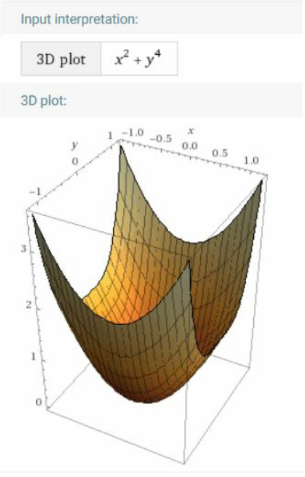
\includegraphics[width=0.9\textwidth]{hesse_semi_definit_funktion_minimum}
      \caption*{\( 0 \) Minimalstelle}
    \end{subfigure}
    \begin{subfigure}[b]{0.3\textwidth}
      \centering
      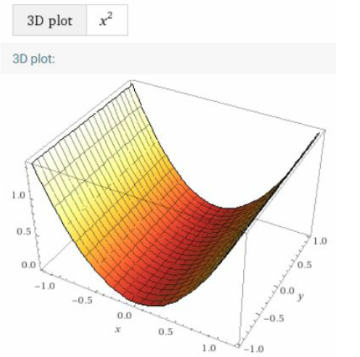
\includegraphics[width=0.9\textwidth]{hesse_semi_definit_funktion_kein_isoliertes_minimum}
      \caption*{\( 0 \) nicht isolierte Minimalstelle}
    \end{subfigure}
    \begin{subfigure}[b]{0.3\textwidth}
      \centering
      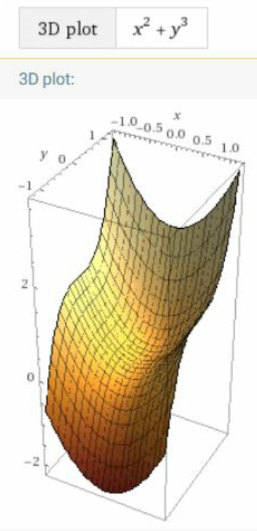
\includegraphics[width=0.9\textwidth]{hesse_semi_definit_funktion_kein_extremum}
      \caption*{\( 0 \) ist keine Extremstelle}
    \end{subfigure}
    \caption{Wolfram Alpha}
  \end{figure}
\end{beispiel*}
\begin{proof}[Beweis von \ref{hinreichende_bedingung_isoliertes_extremum}]
  Setze \( A\definedas H_f(a) \). \texists \( \delta>0 \) \sd \( B_\delta(a)\subset U \). Und somit
  \begin{equation*}
    f(a+h)=f(a)+\scalarproduct{\underbrace{\grad-{f}(a)}_{=0}}{h}+\frac{1}{2}\scalarproduct{h}{Ah}+R_2(h)\quad \forall h\in B_\delta(0)
  \end{equation*}
  mit \( \frac{R_2(h)}{\norm{h}^2}\goesto 0 \) (\( h\goesto 0 \)).
  \begin{equation*}
    \implies \forall \varepsilon>0 \logicspace \exists \tilde{\delta}>0\logicspace (\tilde{\delta}<\delta) \logicspace \text{\sd} \logicspace \abs{R_2(h)}\leq \varepsilon \norm{h}^2\quad \forall h\in B_{\tilde{\delta}}(0)
  \end{equation*}
  \begin{proofdescription}
    \item[\ref{hinreichende_bedingung_isoliertes_minimum}] Sei \( A \) positiv definit. Betrachte \( S=\set{h\in \reals^n|\euclidiannorm{h}=1} \). \( S \) ist abgeschlossen und beschränkt \( \subset \reals^n \) \timplies \( S \) ist kompakt \timplies \( S\ni h\mapsto \scalarproduct{h}{Ah} \) nimmt Maximum und Minimum an (da stetig).
    \begin{equation*}
      \alpha\definedas \inf_{h\in S}\underbrace{\scalarproduct{h}{Ah}}_{\mathclap{>0\logicspace  (\text{VOR})\logicspace (h\neq 0 \text{ wenn }h\in S)}}>0.
    \end{equation*}
    \begin{behauptung*}
      \begin{equation*}
        \scalarproduct{h}{Ah}\geq \alpha\euclidiannorm{h}^2 \quad \forall h\in \reals^n.
      \end{equation*}
    \end{behauptung*}
    \begin{subproof}
      \( h=0\): \checkmark. Sei also \( h\neq 0 \). Setze \( \tilde{h}\definedas\frac{1}{\euclidiannorm{h}}h \).  
      \begin{equation*}
        \implies \tilde{h}\in S\implies \scalarproduct{\tilde{h}}{A\tilde{h}}\geq \alpha.
      \end{equation*}
      Die Behauptung folgt wegen
      \begin{equation*}
        \scalarproduct{\tilde{h}}{A\tilde{h}}=\frac{1}{\euclidiannorm{h}^2}\scalarproduct{h}{Ah}.
      \end{equation*}
    \end{subproof}
    Wähle nun \( \tilde{\delta}>0 \) \sd \( \abs{R_2(h)}\leq \frac{\alpha}{4}\euclidiannorm{h}^2 \) für \( \norm{h}<\tilde{\delta} \).
    \begin{equation*}
      \implies f(a+h)\geq f(a)+\frac{1}{2}\underbrace{\scalarproduct{h}{Ah}}_{\geq \alpha\euclidiannorm{h}^2}-\abs{R_2(h)}\geq f(a)+\underbrace{\frac{1}{4}\alpha\euclidiannorm{h}^2}_{\geq 0}>f(a)\quad \forall \norm{h}<\tilde{\delta},\logicspace  h\neq 0.
    \end{equation*}
    \item[\ref{hinreichende_bedingung_isoliertes_maximum}] Ist \( A \) negativ definit, betrachte \( -f \) und wende \ref{hinreichende_bedingung_isoliertes_minimum} an.
    \item[\ref{hinreichende_bedingung_kein_extremum}] Ist \( A \) indefinit, gibt es in jeder Umgebung \( V \) von \( a \) Punkte \( x,x'\in V \) \sd 
    \begin{equation*}
      f(x)<f(a)<f'(x).
    \end{equation*}
    Es gilt \( v\in \reals^n \), \sd \( \scalarproduct{v}{Av}\defines \alpha >0 \).
    \begin{equation*}
      \implies f(a+th)= f(a)+\frac{1}{2}t^2 a+R_2(tv)
    \end{equation*}
    für \( \abs{t} \) klein genug (\sd \( tv\in B_{\delta}(0) \)). Wähle \( \abs{t}>0 \) so klein, dass zudem \( R_2(tv)\leq \frac{\alpha}{2}t^2 \)
    \begin{equation*}
      \implies f(a+sv)\geq f(a)+\frac{1}{2}s^2\alpha-\abs{R_2(sv)}>f(a)
    \end{equation*}
    für \( 0<s<t \) (\obda \( t>0 \)). 
    
    Genauso: Es gibt \( v\in \reals^n \), \sd \( \scalarproduct{v}{Av}\defines \alpha<0 \)
    \begin{equation*}
      \implies f(x+tv)=f(x)-\frac{1}{2}t^2\abs{\alpha}+R_2(tv)
    \end{equation*}
    für \( \abs{t} \) klein genug (\sd \( tv\in B_{\delta}(0) \)). Wähle \( \abs{t}>0 \) so klein, dass zudem \( \abs{R_2(tv)}\leq\frac{\alpha}{4}t^2 \)
    \begin{equation*}
      \implies f(a+sv)\leq f(a)-\frac{1}{2}s^2\abs{\alpha}+\abs{R_2(sv)}<f(a)\quad \forall 0<s<t\quad (\text{\obda }t>0).
    \end{equation*}
  \end{proofdescription}
\end{proof}
\begin{beispiele*}
  \begin{enumerate}
    \item \( f\maps \reals^2\to \reals \), \( f(x)=x_1^2+x_2^2+2 \), \(\grad-{f}(a)=(2a_1,2a_2)=0\) nur für \( a=0 \).
    \begin{equation*}
      H_f(0)=\begin{pNiceMatrix} 2 & 0 \\ 0 & 2 \end{pNiceMatrix}
    \end{equation*} positiv definit \timplies isoliertes Minimum in \( 0 \).  
    \item \( f\maps \reals^2\to \reals \), \( f(x)=2-x_1^2-x_2^2 \), \( \grad-{f}(a)=-2a=0 \) nur für \( a=0 \). 
    \begin{equation*}
      H_f(0)=\begin{pNiceMatrix} -2 & 0 \\ 0 & -2 \end{pNiceMatrix}
    \end{equation*}
    negativ definit \timplies isoliertes Maximum in \( 0 \).
    \item \( f\maps \reals^2\to \reals \), \( f(x)=2+x_1^2-x_2^2 \), \( \grad-{f}(a)=2a_1-2a_2=0 \) nur für \( a=0 \).
    \begin{equation*}
      H_f(0)=\begin{pNiceMatrix} 2 & 0 \\ 0 & -2 \end{pNiceMatrix}
    \end{equation*}
    indefinit:
    \begin{gather*}
      \textcolor{blue}{\scalarproduct{e_1}{H_f(0)e_1}}=2=-\textcolor{red}{\scalarproduct{e_2}{H_f(0)e_2}}\\
      \textcolor{blue}{f(0+te_1)>f(0)\quad \forall t\neq 0}\\
      \textcolor{red}{f(0+te_2)<f(0)\quad \forall t\neq 0}.
    \end{gather*}
    \begin{figure}[H]
      \centering
      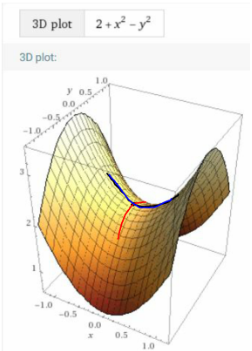
\includegraphics[width=0.5\linewidth]{hesse_indefinit_funktion_sattelflaeche}
      \caption*{Sattelfläche}
      \label{fig:hesse_indefinit_funktion_sattelflaeche}
    \end{figure}
  \end{enumerate}
\end{beispiele*}
\begin{bemerkung*}
  Wie untersucht man in komplizierten Fällen \( H_f(a) \) auf Definitheit? Kennt man die Eigenwerte (\texists wegen Symmetrie!) ist klar: Sind all positiv (negativ), so ist \( H_f(a) \) positiv (negativ) definit, gibt es positive und negative Eigenwerte, so ist sie indefinit. Aber Eigenwerte großer Matrizen sind schwer zu bestimen. Besser geeignet ist
\end{bemerkung*}
\begin{lemma}[aus der AGLA\@: Kriterium von Hurwitz]
  Sei \( A\in \sqmatrices{n}{\reals} \) symmetrisch. Dann ist \( A \) genau dann positiv definit, wenn
  \begin{equation*}
    \Det \explain{\text{Haupt-Minoren von \( A \)}}{\begin{pNiceMatrix} A_{11} & \Cdots & A_{1k} \\ \Vdots &  & \Vdots \\ A_{k1} & \Cdots & A_{kk} \end{pNiceMatrix}}>0\quad \forall k\in \set{1,\dotsc,n}
  \end{equation*}
  und genau dann negativ definit, wenn
  \begin{align*}
    \Det(A_{11})=A_{11}&<0\\
    \Det \begin{pNiceMatrix} A_{11} & A_{12} \\ A_{21} & A_{22} \end{pNiceMatrix}&>0
  \end{align*}
  und dann immer abwechselnd.
\end{lemma}
